\chapter{A systematic approach for identifying shared mechanisms in epilepsy and its comorbidities}
\label{ch:epicom}

\section*{Preface}

The final publication in this thesis describes the curation of a disease-specific knowledge assembly for epilepsy as well as its application in a knowledge-driven analysis of shared mechanisms with \ac{AD}.
It presents an application scenario in which a knowledge-driven approach was used to hypothesize shared pathways between epilepsy and \ac{AD} that might be affected by the drug, carbamazepine, which has been observed through epidemiological studies to have positive therapeutic benefits in both disease contexts.

\vspace*{\fill}

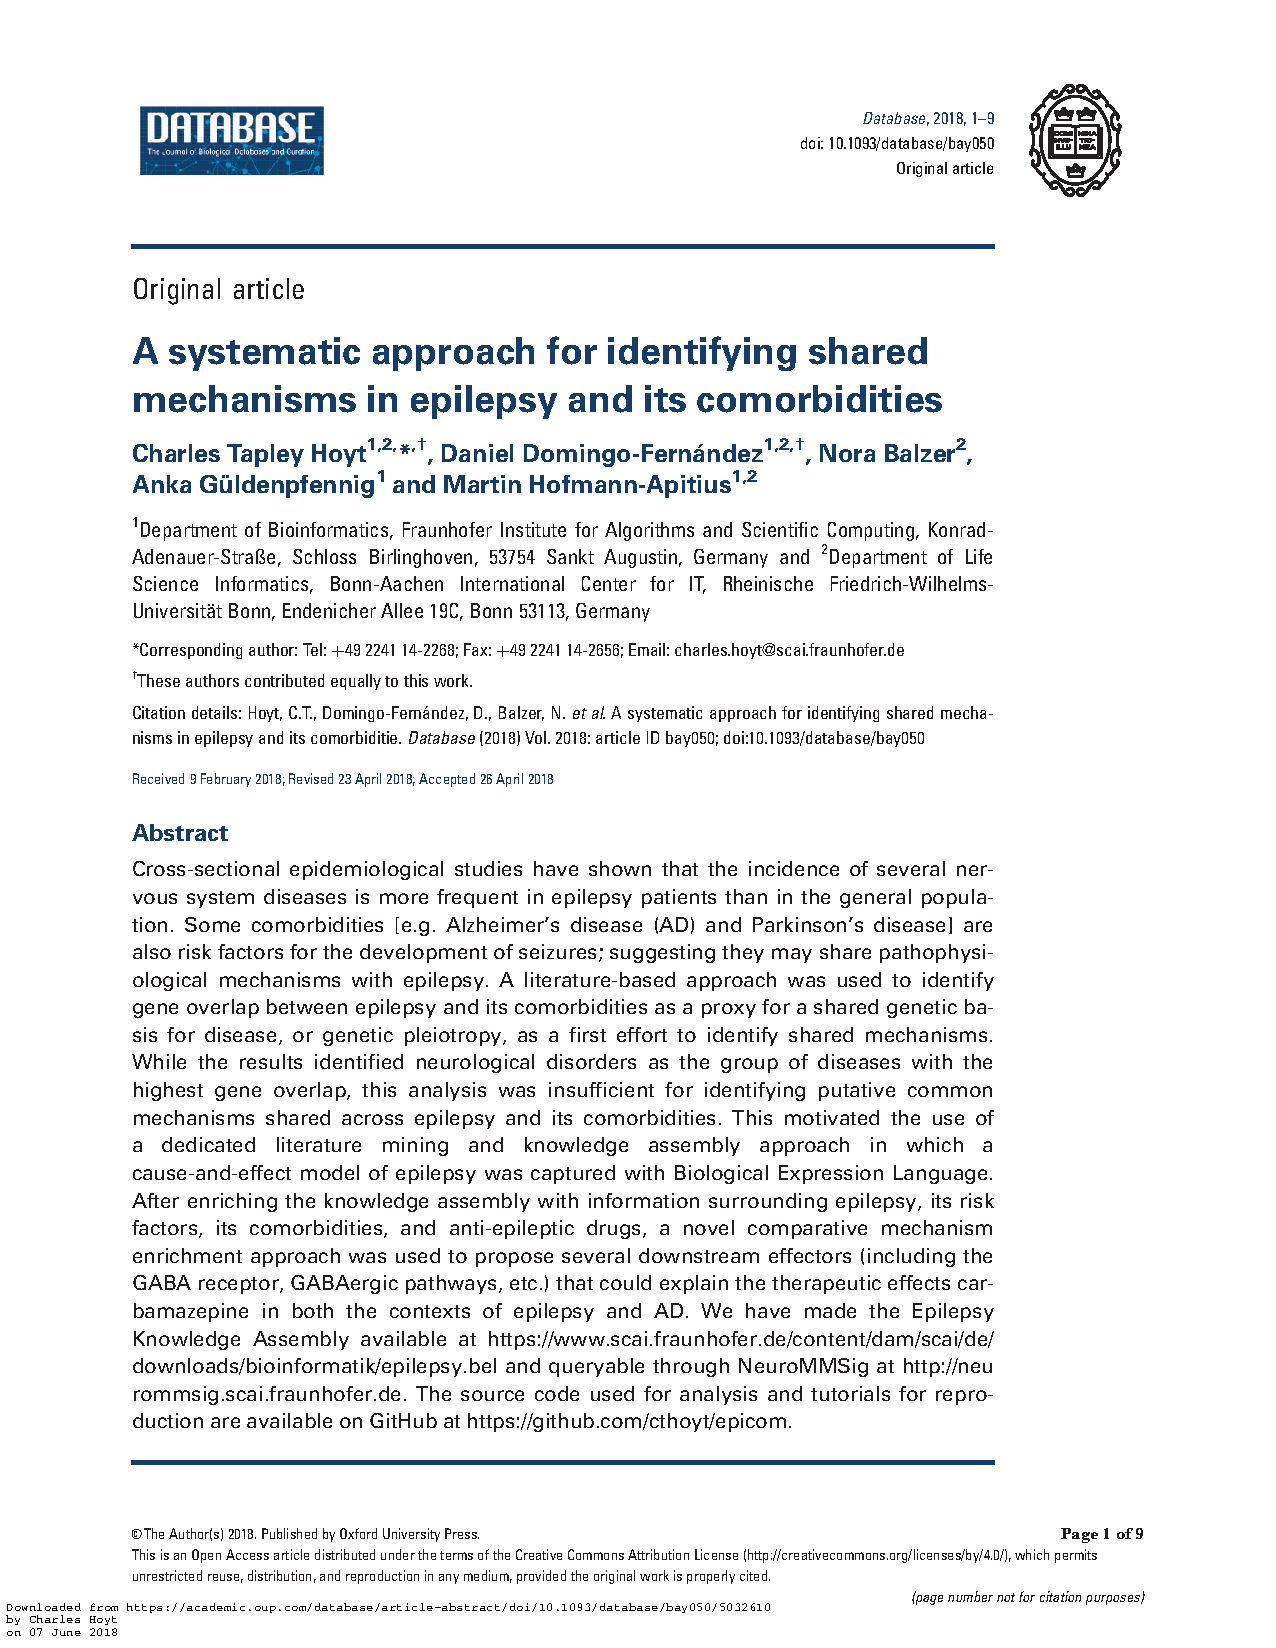
\includepdf[pages={-}]{articles/epicom.pdf}

\section*{Postface}

The analysis presented in this publication ranked disease-specific mechanisms in \ac{AD} and epilepsy that are likely targeted by carbamazepine and ultimately lead to the hypothesis that the GABA-ergic receptor pathway was central to its multi-indication effect.
Importantly, this investigation was advantageous over black-box machine learning models because the underlying knowledge assemblies are self-explanatory and based on publications published in molecular biology and epidemiology.
After, the prospects of applying these techniques in a more automated fashion in order to investigate many more drugs and disease combinations were discussed.
Given the automation enabled by the enrichment methods described in Chapters~\ref{ch:recuration} and~\ref{ch:bio2bel}, this analysis can be more heavily automated to provide new insights as the underlying knowledge assemblies grow and increase in granularity.

Additionally, in the spirit of reproducible and reusable science, the instructions, scripts, and the Epilepsy Knowledge Assembly have been made publicly available in order to enable other scientists to reproduce ours and conduct their own investigations.
